\documentclass[a4paper,11pt]{report}

\usepackage{parskip}
\usepackage[margin=2.54cm]{geometry}
\usepackage[utf8]{inputenc}
\usepackage{graphicx}
\usepackage[table,xcdraw]{xcolor} 
\usepackage{pdfpages}  %to insert pdf documents
\usepackage[draft]{todonotes}
\usepackage{pdflscape}
\usepackage{teresa}  % this is the project-layout style

%Joao Imports
\usepackage{framed,color}
\definecolor{shadecolor}{rgb}{0.9,0.9,0.9}
\usepackage[hidelinks]{hyperref}
\usepackage[hyphenbreaks]{breakurl}
\usepackage{multirow}
\usepackage{subcaption}
\usepackage{amsfonts}
\usepackage{amsmath}
\usepackage{amsthm}
\usepackage{amssymb}

\DeclareMathOperator*{\argmin}{\arg\!\min} 
\DeclareMathOperator*{\argmax}{\arg\!\max}
\usepackage{mathtools}
\usepackage{algorithm}
\usepackage{algorithmic}
\renewcommand{\rmdefault}{phv} % Arial
\renewcommand{\sfdefault}{phv} % Arial
 \usepackage[T1]{fontenc}

\graphicspath{{./}{figures/}}
%\theoremstyle{remark}
\newtheorem{req}{Requirement}
%\newcommand{\citn}{\begin{footnotesize}[cit. needed]\end{footnotesize}}
%\newcommand{\sw}[1]{\textcolor{red}{SW: #1}}
%\newcommand{\jtodo}[1]{\todo[inline]{TODO (Joao): #1}}
\newcommand{\halfrule}{\begin{center}{\rule{0.5\textwidth}{.4pt}}\end{center}}
\newenvironment{draftpts}
{\noindent\ignorespaces\begin{shaded}\begin{center}\footnotesize{DRAFT | Topics to include:}\end{center}\begin{small}}
{\end{small}\end{shaded}\par\noindent\ignorespacesafterend}

\setcounter{secnumdepth}{5}
\setcounter{tocdepth}{5}

%% Adapt the version and code to your deliverable.
%% Those values will appear in the header
\delivcode{D5.3}
\title{Feedback Part 2\\ Integrated Feedback System}
%% Running title
\titlefoot{Feedback Part 2 -- Integrated Feedback System}

\duedate{M30 -  May  31, 2016}
\wpleader{UvA}
\security{Public} %Public or private
\status{Submitted} %Submitted
\delivversion{1.0}



\begin{document}

\maketitle
\makeheader


%%Add a new row with the current version info. 
\begin{documentinfo}

\begin{tabular}{|p{5cm}|p{4cm}|p{5cm}|}
        \hline
        \rowcolor{gray!50}
        Date and Version Number & Author & Comments\\ \hline
        31.05.2016 v1.0 & Jo\~ao Messias \&\hfill Kyriacos Shiarlis & Initial Verson.\\ \hline
\end{tabular}

\end{documentinfo}


\pagebreak
\pagebreak

\tableofcontents

\pagebreak

\listoffigures

\pagebreak

\listoftables

\pagebreak

%\begin{abstract}

%\end{abstract}


\section{Executive Summary}\label{sec:sum}

The TERESA project aims to develop methods that allow a robot to interact effectively with a dynamic social environment. Specifically, we aim to place a semi-autonomous telepresence robot in a day-care center, to allow accessible and seamless communication between its members and remote visitors such as friends and family.\\

 A significant aspect of the project is that cost functions directly related to the movement and behaviour of the robot such as navigation and body pose are partly learned from data instead of being hard-coded. To make this possible, a variety of resources is required such as perception modules, learning algorithms, and of course the data themselves. \\

This deliverable describes the latest advancements 
elements for the TERESA robot through human feedback, in compliance with the 
Description of Work. It discusses:

\begin{itemize}
  \item Learning Algorithms. These are the methods that allow us to associate data from different sensors with feedback from the experiment subjects, into a cost function. We describe the algorithms used and methods for choosing between different design decisions within each algorithm.
  \item Experimentation. We perform experiments with manually 
controlled robots in which the involved subject thinks are autonomous. We describe 
specific instances of such a method, both for social navigation and social conversation scenario, where a 
  large amount of data and human feedback is collected and processed.
  \item Implementation. Using our methods, the collected data and existing algorithms we perform learning in real and simulated robot settings.
\end{itemize}

We present results and progress for all the above topics and explain in what 
ways their respective performance can be improved in the future.

\section{Contributors}\label{sec:cont}

The main contributors to this document are Kyriacos Shiarlis (UvA), Richard Pronk (UvA), Jo\~{a}o Messias (UvA) and Shimon Whiteson (UOXF). The document was reviewed by Luis Merino and Jes\'{u}s Capit\'{a}n (UPO).

\newpage

\section{Introduction}\label{sec:intro}

The technical goal of TERESA is to develop technology that enables a semi-autonomous robot to behave in an acceptable way in social situations. However, it is very hard to determine explicitly what constitutes an “acceptable way” for a robot to behave. Furthermore, imperfections and noise in the sensing and perception systems of the robot might add to the difficutly of designing a social robot. The goal of Work Package 5 is to produce work that overcomes these difficulties and deliver practical methods for improving the social behaviour of the system in a robust manner. This deliverable presents out latest work on learning social policies and cost functions from human interaction. Furthermore it describes both practical and theoretical innovations in the way these cost functions can be integrated.

Firstly in Section ?? we present our latest work on Inverse Reinforcement Learning(IRL) for robotic path planning. In the previous deliverable we presented a new method, Rapidly Exploring Learning Trees, which allows learning of Rapidly Exploring Random Trees, from human demonstrations. I this deliverable we present an extension of the method that takes into account the kinodynamic constraints of the robot and we deploy the method on real data collected using the TERESA robot. 

Section ?? outlines a method that uses data of human demonstrations coupled with Deep Neural Networks, that allows the robot to learn body pose policies. Such policies determine for example how the robot should possition itself in the presence of an interaction target and an interaction group as well as how it should react to their movement.

Next in Section ?? we demonstrate how the cost functions learned using human feedback in Deliverable 5.3, can be integrated with the system detailed in Section ??. This is done using a novel hierarchical Neural Network architectures that Reinforcement Learning and Supervised Learning simultaneously. We further present an evaluation that shows that the robot can learn to replicate the demonstrated behaviour while at the same time perform well with respect to the given cost function.  

Finally in Section ??, we describe a more theoretical approach to cost function integration. This is based on...MOPOMDP...

\pagebreak


\section{Rapidly Exploring Learning Trees}
\label{sec:rrt-iros}
As we have seen in previous sections, IRL is a general method and can be used in conjunction with any decision-making task. When applied to robotics however, IRL falls under the more general umbrella term of learning from demonstration (LfD) \cite{argall2009survey}. LfD is of great interest to roboticists because it can avoid the need for tedious manual programming of complex behaviours. While most LfD methods rely on supervised learning to directly learn policies, certain approaches, such as IRL and the closely related field of inverse optimal control (IOC) \cite{kalman1964linear} instead learn \emph{cost functions} from demonstration. These cost functions are then used to \emph{plan} the robot's behaviour. 

Cost functions tend to be more general and robust to changes in the environment such as friction in a manipulator's joints. A robot trained in a supervised manner has less chance of adapting than one that has been trained using IRL or IOC because the cost function remains unchanged. In addition, cost functions are thought to be more succinct representations of the aims of the agent \cite{abbeel2004apprenticeship}. %For example, an agent that whose aim is to get as fast as possible to a goal location. The policy for such an agent will be much harder to interpret when compared to its cost function. 

However, inverse methods also have practical limitations. IRL for example requires modeling the task as a Markov decision process (MDP), which is typically impractical in robotics, for several reasons.  Firstly, an MDP assumes full observability. Secondly, planning in an MDP, which IRL methods must do repeatedly, is costly, especially in continuous and high-dimensional domains. Finally, the lack of scalability and the assumption of full observability prohibit the natural modeling of important factors such as kinodynamic constraints. Applying IRL to the real setting of the TERESA robot, therefore requires the invention of new methods that are more applicaple to robotics. 

Several researchers have proposed replacing the planning step in IRL with more convienient planners, e.g., Maximum Margin Planning (MMP)~\cite{ratliff2006maximum} uses A$^*$ search for planning. This avoids the need to do all the planning in advance, as is typical when solving an MDP. It also avoids the need to model all aspects of the environment since the robot can quickly replan its trajectory to account for uncertainty. However, deterministic search methods such as A$^*$ require discretisation of the state space, and quickly run into scalability problems as the discretisation becomes finer. Furthermore, this discretisation again ignores kinodynamic constraints.

In path planning, Rapidly Exploring Random Trees (RRTs)~\cite{lavalle1998rapidly} are popular because they cope well with continuous and high-dimensional domains and can elegantly handle kinodynamic constraints. The RRT$^*$ algorithm \cite{karaman2011sampling}, which extends RRTs to incorporate a cost function, is especially effective. However, the cost functions used by RRT$^*$ are typically simple and hand-coded and, to our knowledge, no methods have been developed to learn RRT$^*$ cost functions from demonstrations.

In this section, we propose Rapidly Exploring Learning Trees (RLT), which learns RRT$^*$ cost functions from demonstration. Specifically we modify Maximum Margin Planning to use RRT$^*$ as a planner. Furthermore, we propose a caching scheme that greatly reduces the computational cost of this approach. RLT requires no additional planner assumptions other than those inherent in RRT$^*$, making it particularly easy to implement. 

We evaluate RLT on real and simulated data from a social navigation scenario. The results demonstrate that RLT achieves better performance at lower computational cost than methods that learn path planning cost functions for deterministic planners.

\subsection{Related Work}

Substantial research has applied IRL to robotics \cite{henry2010learning,abbeel2008apprenticeship,vasquez2014inverse}. Because of the need to model the environment as an MDP, researchers usually discretise the state-action space. This introduces several key limitations. First, the size of the state-action space encountered in robotics is often prohibitive for such models. Second, the specific kinodynamic constraints of the robot cannot be easily be expressed by such representations, as they introduce non-Markovian dynamics. 

% \ks{Depending on the state-action space discretisation, past actions can infuence how easy it is to move to any a subsequent state. However the transition function only considers only one action in the past, and it is therefore an expectation over possible past configurations. As a result it tends to give the wrong probability distribution over next states for the actual physical system. Do I have to explain this in detail? Maybe Joao has a citation from his research?}

To apply IRL to more realistic situations, researchers usually try to replace the MDP model while retaining the main idea behind IRL, i.e., learning the underlying cost function of a planner using data from demonstrations. Maximum Entropy IRL \cite{ziebart2010modelingthesis} works in domains with linear continuous dynamics with the optimal controller being a Linear-Quadratic Regulator. Since linear dynamics are hard to come by in robotics, \cite{2012-cioc} considers locally linear aproximations. These bring about locally consistent rewards and achieve good performance in a range of tasks that were previously too hard for MDPs. However, the optimisation of the cost function using such planners is not guaranteed to be optimal. As our method is based on an RRT$^*$ planner, it is asymptotically optimal.

Other approaches to the problem use hybrid planners. Inverse Optimal Heuristic Control \cite{ratliff2009inverse} models the long-term goals of the agent as a coarse state MDP, to ensure tractability, while using supervised learning to determine the local policy of the agent at each state. Graph-Based IOC \cite{byravan2015graph} uses discrete optimal control on a coarse graph and the actual path is executed using local trajectory optimisation techniques such as CHOMP \cite{ratliff2009chomp}, which would otherwise suffer from local minima. The method is effective in robotic manipulation tasks with many degrees of freedom.  However, these methods employ complex and domain-specific planning formulations that are not suitable for all robotics tasks. The method presented here employs widely used planners, making it versatile and easy to implement. 

Another more recent graph-based concept is that of Adaptive State Graphs \cite{okallearning}, which build a controller graph before doing any learning. This controller graph is akin to \emph{options} in semi-Markov decision processes, and allows for a more flexible representation of the state-action space. However, the controller used to learn the underlying cost function is not the same as the one used to execute the robot's behaviour. This can have an adverse effect since an implicit assumption of IRL is that the demonstration paths came from the same planner that we use during learning. This planner has specific representations, such as discretisation and parameters such as the discount factor. If these change, different policies arise. As a result a path that was optimal under a certain planner ceases to be optimal under another.

RLT$^*$ can also be viewed as a graph-based, or rather tree-based, approach. Instead of building a controller graph first and then using different controllers to optimise trajectories, RLT$^*$ builds a controller tree on the fly. RLT$^*$ however uses the exact same planner during learning and execution.


\subsection{Background}
We begin with background on path planning and inverse reinforcement learning for path planning.

\subsubsection{Path Planning \label{subsec:path_planning}}
Path planning occurs in a space $\mathcal{S}$ of possible configurations of the robot. A configuration $s \in \mathcal{S}$ is usually continuous, and often represents spatial quantities such as position and orientation. A path planner seeks an obstacle-free path $\zeta_{o,g} = (s_1,s_2,s_3$ $\ldots,s_{l_{\zeta}}) $ of length $l_{\zeta}$, from an initial configuration $o = s_1$ to a goal configuration  $g =s_{l_{\zeta}}$. When the initial and goal configurations are implied, we refer to a path as $\zeta$.

Because there could be several paths to the goal, path planners typically employ a \emph{cost functional}, $C(\zeta)$ often defined as the sum of the costs between two subsequent configurations in a path $c(s_i,s_j)$. The total cost $C(\zeta)$ is therefore the sum of the individual costs along the path, i.e.,
\begin{equation}
	C(\zeta) = \sum_{i=1}^{l_{\zeta}-1} c(s_i,s_{i+1}).
\end{equation}
This cost functional is similar to the one encountered in optimal control as well as to value functions used in reinforcement learning. Given the cost functional, the path planner seeks an optimal path $\zeta^*$, which satisfies,
\begin{equation}
 	\zeta^*_{o,g} = \argmin_{\zeta_{o,g} \in Z_{o,g}} C(\zeta), \label{eq:back_plan}
\end{equation}
where $Z_{o,g}$ is the set of all possible paths such that $s_1 = o, s_{l_\zeta} = g$.

Many path planning algorithms discretise $\mathcal{S}$ and use graph search algorithms like A$^*$ to find the optimal path. Under mild assumptions, these approaches are guaranteed to find the best path on the graph, but not in $\mathcal{S}$. However, they scale poorly in the size of $\mathcal{S}$, as larger and larger graphs are required. Furthermore, such methods do not address kinodynamic constraints, i.e., they assume that every configuration on the graph is accessible from a neighbouring one. 

These drawbacks motivate \emph{sample-based} path planning algorithms such as RRT$^*$. Instead of building a graph and then searching it, RRT$^*$ builds a tree on the fly and keeps track of the current best path. This tree can be grown in a way that respects kinodynamic constraints. Furthermore, a sampled-based approach can quickly find good, but not optimal, paths in large configuration spaces.

%  RRT$^*$ is also asymptotically optimal, i.e., it is guranteed to find an optimal path in $\mathcal{S}$ as the sampling time goes to infinity. Many variants of RRT$^*$ provide improved performance and faster convergence in practice by, for example, heuristically shriking the sampling space \cite{gammell2014informed}.

% The most significant difference between A$^*$ and RRT$^*$ is that while former is deterministic, the latter is probabilistic. It is important to understand how this distinction affects learning.

A$^*$ can solve \eqref{eq:back_plan} for a subset $\tilde{Z}_{o,g} \in  Z_{o,g}$ that is determined by its resolution (discretisation). RRT$^*$, for a given time budget $T$, also minimises a subset but in this case $\tilde{Z}_{o,g}$ is determined by the randomly sampled points. As $T \rightarrow \infty$, RRT$^*$ minimises over the entire $Z_{o,g}$, i.e., it is asymptotically optimal. In other words, the RRT$^*$ is asymptotically optimal as a function of sampling time and A$^*$ is asymptotically optimal as a function of resolution. %This distinction will become very important when we attempt to learn cost functions for these planners in the next section.

\subsubsection{IRL for Path Planning \label{subsec:inverse_problem}}
Path planning involves finding a (near) optimal path to the goal given a cost function. In the inverse problem, we are given example paths and must find the cost function for which these paths are (near) optimal.  The example paths comprise a dataset $\mathcal{D} = (\zeta^1_{o_1,g_1},\zeta^2_{o_2,g_2}...\zeta^D_{o_D,g_D})$ where $\zeta^i_{o_i,g_i}$ is an example path with initial and final configurations $o_i,g_i$ respectively. We assume the unknown cost function is of the form,
\begin{equation}
	c(s_i,s_j) = \mathbf{w}^T \mathbf{f}(s_i,s_j), \label{eq:inner_prod}
\end{equation}
where $\mathbf{f}(s_i,s_j)$ is a $K$-dimensional vector of features that encode different aspects of the configuration pair and $\mathbf{w}$ is a vector of unknown weights to be learned. Since $\mathbf{w}$ is independent of the configuration, we can express the total cost of the path in a parametric form:

\begin{equation}
	C(\zeta) = \mathbf{w}^T\sum_{i=0}^{l_{\zeta}-1} \mathbf{f}(s_i,s_{i+1}) := \mathbf{w}^T \mathbf{F}(\zeta),
\end{equation}
where $\mathbf{F}(\zeta)$ is the \emph{feature sum} of the path.

While many formulations of the inverse problem exist, the general idea is to find a weight vector that assigns less cost to the example paths than all other possible paths with the same initial and goal configuration.  This can be formalised by a set of inequality constraints:

\begin{equation}
	C(\zeta^i_{o_i,g_i}) \leq  C(\zeta) \quad \forall \zeta \in Z_{o_i,g_i}  \quad \forall i. \label{eq:const1}
\end{equation}
The constraint is an inequality because $Z_{o,g}$ contains only paths available to the planner and thus may not include the example path $\zeta^i_{o_i,g_i}$.
$Z_{o_i,g_i}$ can be large but if we have an optimisation procedure that solves \eqref{eq:back_plan}, it is enough to satisfy, 
\begin{equation}
	C(\zeta^i_{o_i,g_i}) \leq \min_{\zeta \in Z_{o_i,g_i}} C(\zeta) \quad \forall i, \label{eq:const}
\end{equation}

Ratliff et al.\ \cite{ratliff2006maximum} propose a maximum margin variant of \eqref{eq:const} by introducing a margin function $L_i(\zeta)$ that decreases the cost of the proposed path $\zeta$ if is dissimilar to $\zeta^i_{o_i,g_i}$. For example, $L_i(\zeta)$ could be $-1$ times the number of configurations in the demonstration path not visited by $\zeta$. The full optimisation formulation of Maximum Margin Planning is as follows.

\begin{equation}
	\argmin_{\mathbf{w},\tau} \frac{1}{2}||\mathbf{w}||^2 + \frac{\lambda}{D} \sum_i \tau_i \label{eq:mas_marg}
\end{equation}
\begin{equation}
	\text{s.t.} \quad C(\zeta^i_{o_i,g_i}) - \tau_i \leq \min_{\zeta \in Z_{o_i,g_i}} C(\zeta) + L_i(\zeta) \quad \forall i,
\end{equation}
where $\tau_i$ are slacks that can be used to relax the constraints. Rearranging the inequality in terms of the slacks we get:

\begin{equation}
	 \quad C(\zeta^i_{o_i,g_i}) - \min_{\zeta \in Z_{o_i,g_i}} C(\zeta) + L_i(\zeta)  \leq \tau_i  \quad \forall i.
\end{equation}
Consequently, the $\mathbf{w}$ minimising:
\begin{equation}
	\frac{1}{2}||\mathbf{w}||^2 + \frac{\lambda}{D} \sum_i \big( C(\zeta^i_{o_i,g_i}) - \min_{\zeta \in Z_{o_i,g_i}}\big(C(\zeta) + L_i(\zeta)\big) \big) \big. \label{eq:unconstrained}
\end{equation}
is equivalent to that which minimizes \eqref{eq:mas_marg}, i.e., the slacks are tight.
The minimum can be found by computing a subgradient and performing gradient descent on the above objective:
\begin{equation}
	\nabla_{\mathbf{w}} =\mathbf{w} +  \frac{\lambda}{D} \sum_{i=0}^D F(\zeta^i_{o_i,g_i}) - F(\tilde{\zeta}^*_{o_i,g_i}), \label{eq:update1}
\end{equation}
where,
\begin{equation}
	\tilde{\zeta}^*_{o_i,g_i} = \argmin_{\zeta \in Z_{o_i,g_i}} C(\zeta) + L_i(\zeta). \label{eq:augmented_max}
\end{equation}

The inverse problem can therefore be seen as an iterative procedure, that first solves \eqref{eq:augmented_max} in the inner loop while keeping the weights constant. Based on that solution, it updates the weights using \eqref{eq:update1} in the outer loop. The weights at convergence represent the cost function that is used to plan the future behaviour of the agent. In \cite{ratliff2006maximum}, A$^*$ search was used for planning in the inner loop, assuming that the domain contained acyclic positive costs. In this work, we make the same assumptions but develop methods that use RRT$^*$ for planning.

\subsection{Method}
	In this section, we propose Rapidly Exploring Learning Trees (RLT$^*$).  We first propose a generic extension to the maximum margin approach that we call Approximate Maximum Margin Planning.  We then show how an implementation of this approach with an RRT$^*$ planner and a novel caching scheme yields RLT$^*$.

	% \subsection{Feature Sums and Sampled Based Planners}
	% 	Feature sums, $F(\zeta)$, can be seen as the  `fingerprints' of paths, and their definition is of crucial importance in the inverse problem. When planning on a fixed graph, like in the case of MDPs or A$^*$ search, it is easy to define the feature sums as the \emph{edge} costs on the graph. Furthermore if planning in continous domains we may consider integrals along the path. In RRT's however the tree that is being built has neither a fixed structure, nor an analytical form. Thus, the first step towards learning RRT$^*$ cost functions from demonstration is to come up with a reasonable approximation of $F(\zeta)$ for a path. This approximation must be consistent with the definition of the cost for a configuration pair. One such definition for cost is as follows.
	% 	\begin{equation}
	% 		c(s_i,s_j) = \frac{c(s_i)+c(s_j)}{2}d_{s_i,s_j}
	% 	\end{equation}
	% 	Where $c(s_i)$ is a cost function defined over a single configuration and $d_{s_i,s_j}$ is a measure of distance between the two configurations. For example if we consider configurations to be points in Eucledian space then $d_{s_i,s_j}$ can be the eucledian distance. Noting that the costs and features are related by \eqref{eq:inner_prod} for a single feature $f_k$ we have,

	% 	\begin{equation}
	% 		f_k(s_i,s_j) = \frac{f(s_i)+f(s_j)}{2}d_{s_i,s_j}
	% 	\end{equation}
	% 	Following this definition feature sum calculation along a candidate path is trivial,
	% 	\begin{equation}
	% 		F(\zeta) = \sum_{i=0}^{\zeta_l-1} \frac{\mathbf{f}(s_i)+\mathbf{f}(s_{i+1})}{2}d_{s_i,s_{i+1}}
	% 	\end{equation}

\subsubsection{Approximate Maximum Margin Planning \label{subsec:ammp}}

		In Section \ref{subsec:inverse_problem}, we showed how the multiple constraints of \eqref{eq:const1} could be reduced to a single constraint for each demonstration in \eqref{eq:const}. However, given a finite time budget $T$, a sample-based planner like RRT$^*$ minimises, not over the full set of paths $Z_{o,g}$, but over a randomly sampled $\tilde{Z}_{o,g}$. Thus, we can modify \eqref{eq:const}, and demand that our cost function satisfies,
\begin{equation}
	C(\zeta^i_{o_i,g_i}) \leq \min_{\zeta_{o_i,g_i} \in \tilde{Z}_{o_i,g_i}} C(\zeta) \quad \forall i. \label{eq:const_rrt}
\end{equation}
	As the planning budget $T$ increases, the sample-based planner samples lower cost paths, making this inequality harder to satisfy. Assuming $\tilde{Z}_{o_i,g_i}$ is constant, we can rewrite \eqref{eq:unconstrained} as:

	\begin{equation} \frac{1}{2}||\mathbf{w}||^2 + \frac{\lambda}{D} \sum_i \big( C(\zeta^i_{o_i,g_i}) - \min_{\zeta \in \tilde{Z}_{o_i,g_i}}\big(C(\zeta) + L_i(\zeta)\big) \big). \label{eq:unconstrained_rrt}
	\end{equation}
	This gives rise to an approach we call Approximate Maximum Margin Planning (AMMP), which is similar  to the one described in Section \ref{subsec:inverse_problem}, with the crucial difference that the planning step is executed by a sample-based planner and not a deterministic one, like A$^*$. An important consequence is that $\tilde{Z}_{o_i,g_i}$ now changes every time we invoke the sample-based planner. As a result, AMMP can be thought of as a smart way of sampling the \emph{constraints} that we want our cost function to satisfy. 


\subsubsection{Rapidly Exploring Learning Trees \label{subsec:cached}}

A simple way to construct a concrete algorithm from AMMP is to use RRT$^*$ as the sample-based planner.  However, this results in a computationally expensive algorithm, which calls the planner $I\times|D|$ times over $I$ iterations given a dataset of size $|D|$.  Since planning is typically expensive, it is crucial to find a more efficient approach.

In this section, we propose Rapidly Exploring Learning Trees (RLT$^*$), which implements AMMP with an RRT$^*$ planner but uses a caching scheme to achieve computational efficiency.

Two of the most costly operations of RRT$^*$ are 1) finding the nearest neighbour to a newly sampled point and 2) finding the radius-neighbours of a newly created vertex in the tree \cite{karaman2011sampling}. However, a key observation is that neither of these procedures depend on the cost function used by the planner. Thus,  RRT$^*$ can be split in two independent steps. 

	The first step is described in Algorithm \ref{alg:rrt_cache}, which takes as input $p$, the number of points to randomly sample from free space; $s_{init}$, the initial point; and $\eta$, the steer step size. For each randomly sampled point $s_{rand}$, we find the nearest neighbour, $s_{nearest}$, from the set of points in the vertex set $V$. We then create a new configuration point $s_{new}$ by steering from $s_{nearest}$ to $s_{rand}$. Next, we query the radius neighbours of $s_{new}$ at a radius determined by  $\min\{\gamma_{RRT^*}(\frac{\log(|V|)}{|V|})^{\frac{1}{d}},\eta\}$. Here, $d$ is the dimensionality of $S$, and $\gamma_{RRT^*}$ is a constant based on the volume of free space (see \cite{karaman2011sampling}). The points $s_{new}$, $s_{nearest}$ and the set $S_{near}$ are stored together in the map $P$, which we call the \emph{point cache}, and is returned at the end of the procedure. This algorithm turns the sampling process of RRT$^*$  into a preprocessing step. Consequently, the expensive \texttt{Nearest} and \texttt{Near} procedures only need to be repeated $|D|$ times instead of $I\times|D|$ times.

	\begin{algorithm}
		 \algsetup{linenosize=\small}
 	\scriptsize

	\caption{\texttt{planCachedRRT$^*$}($P$,$s_{init}$,$c()$)}

	 \label{alg:plan_cached}

	\begin{algorithmic}[1]
	\STATE $E \gets \emptyset$
	\STATE $V \gets {s_{init}}$
	\FOR{$i=0 \dots |P| $}
	\STATE $s_{nearest} \gets P\{s_{nearest}^i\}$
	\STATE $s_{new} \gets P\{s_{new}^i\}$
	\STATE $S_{near} \gets P\{S_{near}^i\}$
	\STATE $V\gets V \cup s_{new}$
	\STATE $s_{min}\gets s_{nearest}$
	\STATE $c_{min}\gets \texttt{Cost}(s_{nearest}) + c(s_{nearest},s_{new})$
	\FOR{$s_{near} \in S_{near} $}
	\STATE $c_{near} \gets \texttt{Cost}(s_{near}) + c(s_{near},s_{new})$
	\IF {\texttt{CollisionFree}($s_{near},s_{new}$) and  $c_{near}<c_{new}$}
	\STATE $s_{min} \gets s_{near}; c_{min}\gets c_{near}$
	\ENDIF
	\ENDFOR
	\STATE $E \gets E \cup \{(s_{min},s_{new})\} $
	\FOR{$s_{near} \in S_{near} $}
	\STATE $c_{new} \gets \texttt{Cost}(s_{near}) + c(s_{near},s_{new})$
	\IF {\texttt{CollisionFree}($s_{near},s_{new}$) and  $c_{new}<\texttt{Cost}(s_{near})$}
	\STATE $s_{parent} \gets \texttt{Parent}(s_{near})$
	\STATE $E \gets E  \smallsetminus {(s_{parent},s_{near})} \cup {(s_{new},s_{near})} $
	\ENDIF
	\ENDFOR
	\ENDFOR
	\STATE $\zeta_{min} \gets \texttt{minCostPath}(V,E,c())$
	\RETURN $\zeta_{min}$
	\end{algorithmic}
	\end{algorithm}


	\begin{algorithm}
	 \algsetup{linenosize=\small}
 	\scriptsize
	\caption{\texttt{cacheRRT}($p$,$s_{init}$,$\eta$)}
	\label{alg:rrt_cache}
	\begin{algorithmic}[1]
	\STATE $P \gets \emptyset$ \hfill \COMMENT{Initialise the point cache}
	\STATE $V \gets {s_{init}}$
	\FOR{$i=0 \dots p $}
	\STATE $s_{rand} \gets SampleFree_i$
	\STATE $s_{nearest} \gets \texttt{Nearest}(V,s_{rand})$
	\STATE $s_{new} \gets \texttt{Steer}(s_{nearest},s_{rand})$
	\STATE $S_{near} \gets \texttt{Near}(V,{s_{new}},\min\{\gamma_{RRT^*}(\frac{\log(|V|)}{|V|})^{\frac{1}{d}},\eta\})$ 
	\STATE $V\gets V \cup s_{new}$
	\STATE $P \gets P \cup \{s_{new},S_{near}\}$
	\ENDFOR
	\RETURN $P$

	\end{algorithmic}
	\end{algorithm}

The output of Algorithm \ref{alg:rrt_cache} is input to Algorithm \ref{alg:plan_cached}, which resembles wiring and re-wiring procedures in RRT$^*$ \cite{karaman2011sampling}, and returns a minimum cost path to the goal. An important difference, however, is that the vertices of the tree and their neighbours at each iteration are already known and contained within the point cache. This speeds computation while keeping consistency between the planners used during learning and final execution. As learning proceeds and the cost function changes, so does the wiring of this tree; however, the points involved do not change.

Algorithm \ref{alg:ammp} describes Rapidly Exploring Learning Trees (RLT$^*$), which uses  Algorithms \ref{alg:rrt_cache} and \ref{alg:plan_cached}. First, we initialise the weights, either randomly or using a cost function that simply favours shortest paths. Then, for each datapoint $\zeta_i$, we calculate feature sums and run \texttt{cacheRRT}. The main learning loop involves cycling through all data points and finding the best path under a loss-augmented cost function. The feature sums of this path are calculated and subsequently the difference with the demonstrated feature sums is computed. At the end of each iteration, an average gradient is calculated and the cost function is updated. At convergence, the learned weights are returned.

	\begin{algorithm}
	 \algsetup{linenosize=\small}
  	\scriptsize
	\caption{\texttt{RLT$^*$}($D,p,\eta,\lambda,\delta$)\label{alg:ammp}}
	\begin{algorithmic}[1]
	\STATE $\mathbf{w} \gets \texttt{initialiseWeights}$
	\STATE $\mathbf{\tilde{F}} \gets \emptyset$
	\STATE $R \gets \emptyset$
	\FOR{$\zeta^i \text{ in } D$}
	\STATE $\tilde{F}_{\zeta^i} \gets \texttt{FeatureSums}(\zeta^i)$
	\STATE $\mathbf{\tilde{F}} \gets \mathbf{\tilde{F}} \cup \tilde{F}_{\zeta^i}$
	\STATE $r_i \gets \texttt{cacheRRT}(p,s_{init}^{\zeta^i},\eta)$
	\STATE $R \gets R \cup r_i $
	\ENDFOR
	\REPEAT
	\STATE $\nabla_{\mathbf{w}}\gets 0$
	\FOR{$ \zeta^i \text{in } D $}
	\STATE $c() \gets \texttt{getCostmap}(\mathbf{w}) + L(\zeta^i)$ 
	\STATE $r_i \gets R\{i\}$ ;	$\tilde{F}_i \gets \mathbf{\tilde{F}}\{i\}$ 
	\STATE $\zeta \gets \texttt{planCachedRRT}^*(r_i,x^i_{init},c())$
	\STATE $F_i \gets \texttt{FeatureSums}(\zeta)$
	\STATE $\nabla_{\mathbf{w}} \gets \nabla_{\mathbf{w}} + \tilde{F}_i - F_i $
	\ENDFOR
	\STATE $\nabla_{\mathbf{w}} \gets \mathbf{w} + \frac{\lambda}{|D|}\nabla_{\mathbf{w}} $
	\STATE $\mathbf{w} \gets \mathbf{w} - \delta\nabla_{\mathbf{w}} $
	\UNTIL{convergence}
	\RETURN $V,E$

	\end{algorithmic}
	\end{algorithm}

	% \STATE $\widetilde{\mu}^{\mathcal{D}} \gets \mathtt{empiricalFE}(\mathcal{D})$\hfill \COMMENT{using \eqref{eqn:empirical_fe}}
	% \STATE $\widetilde{\mu}^{\mathcal{F}} \gets \mathtt{empiricalFE}(\mathcal{F})$ 
	% \STATE $P_{\mathcal{D}}^{s_1} \gets \mathtt{initialStateDistribution}(\mathcal{D})$
	% \STATE $P_{\mathcal{F}}^{s_1} \gets \mathtt{initialStateDistribution}(\mathcal{F})$
	% \STATE $w^{\mathcal{F}}_k\gets 0\quad\forall k\in\{1,\ldots,K\}$
	% \REPEAT
	% \STATE $R(s,a) \gets (w^{\mathcal{D}}+w^{\mathcal{F}})^T\phi(s,a)\quad\forall s\in\mathcal{S},a\in\mathcal{A}$
	% \STATE $\pi \gets \mathtt{softPlan}(\mathcal{S},\mathcal{A},T,R)$\hfill\COMMENT{using \eqref{eq:soft_backup}}
	% \STATE $\mu^\pi|_{\mathcal{D}} = \mathtt{calculateFE}(\pi,T,P_{\mathcal{D}}^{s_1})$
	% \STATE $\mu^\pi|_{\mathcal{F}} = \mathtt{calculateFE}(\pi,T,P_{\mathcal{F}}^{s_1})$
	% \STATE $w^{\mathcal{D}} \leftarrow w^{\mathcal{D}} - \alpha (\mu^\pi|_{\mathcal{D}} - \widetilde{\mu}^{\mathcal{D}})$
	% \STATE $w^{\mathcal{F}} \leftarrow \frac{(\mu^\pi|_{\mathcal{F}} - \widetilde{\mu}^{\mathcal{F}})}{\lambda}$

	% \IF {$\lambda > \lambda_{min}$}
	% \STATE $\lambda \leftarrow \alpha_{\lambda}\lambda$
	% \ENDIF
	% \UNTIL{convergence}
	% \RETURN $R,\pi$


For RRT$^*$ the dependance of $\tilde{Z}_{o_i,g_i}$ on the time budget T is very hard to quantify since it also depends on the size and nature of $S$ as well as the cost function we are using -which also changes with every iteration. For this reason, in this work we resort to an experimental assesment of the ability of RRT$^*$ to sample the right constraints at every iteration of RLT$^*$ and hence allow the learning of a cost function from a set of demonstrated paths.


\subsection{Experiments}
In this section, we experimentally compare RLT$^*$ to the original MMP algorithm implemented using an A$^*$ planner and ablated version of RLT$^*$ that does not use caching, using a simulated version of the TERESA robot. 
	
	Our experiments take place in the context of social navigation. IRL has been widely used in this setting \cite{okallearning,henry2010learning,vasquez2014inverse} because it is usually infeasible to hard-code the cost functions that a planner should use in complex social situations. Having the ability to quickly and effectively learn social navigation cost functions from demonstration would be a major asset, not only for the TERESA robot but also for robots that operate in crowded environments such as airports \cite{triebel2015spencer}, museums \cite{thrun1999minerva}.
	
\subsubsection{Setting}
	Our experiments take place in a randomly generated social environment, shown in Figure \ref{fig:exp_setting}. Every arrow in the figure represents a person's position and orientation. The robot is given the task of navigating from one point in the room to another. While it is aware of the orientation and position of different people, it has no idea on how to trade off reaching the target quickly with avoiding people and obstacles, i.e., the cost function is unknown. Instead, the robot is given a dataset of demonstrations $D$. Each demonstration $\zeta_i$ is a set of configurations $s = (x,y)$ representing positions of the robot in the configuration space and each demonstration takes place for a different random configuration of the social environment, i.e., the people are at different positions and orientations every time. The task of the robot is to, using $D$, extract a cost function based on different features of the environment, which in turn would allow it to behave socially in future tasks. These simulated settings are similar to the ones enountered by the TERESA robot during normal operation. Furthermore these simulations utilise a faithful Gazebo \footnote{www.gazebosim.org} model of the TERESA robot.

  The features involved in our experiments can be divided in three sets. The first set encodes proxemics to the people present in the scene. These are represented by three Gaussian functions of different means and diagonal covariances around each person. The second set of features encodes the distance from the target location using linear, exponential and logarithmic functions. The third set encodes the obstacle cost using a stable function of the reciprocal of the distance from the nearest obstacle. Figure \ref{fig:cost_f} shows an example cost function over the whole configuration space for the configuration in Figure \ref{fig:exp_setting}. We use different functions for human and target proximity, to allow for more degrees of freedom when modeling the underlying cost function. Sufficient regularisation ensures that that the model does not overfit.


	\begin{figure}[tbh]
%	\hspace{-5cm}
  \centering
      \begin{subfigure}[b]{0.435\columnwidth}
	\hspace{5mm}
    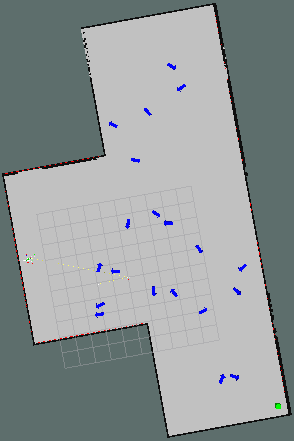
\includegraphics[width=0.7\textwidth]{figures/people.png}
    \caption{Example setting }
    \label{fig:exp_setting}
  \end{subfigure}
  \hspace{10mm}
  \begin{subfigure}[b]{0.435\columnwidth}
  \hspace{4mm}
    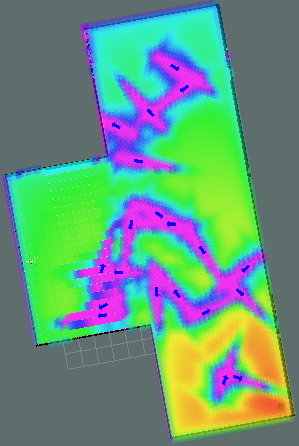
\includegraphics[width=0.7\textwidth]{figures/cost_f.png}
    \caption{Cost function}
    \label{fig:cost_f}
  \end{subfigure} 

  %\vspace{-3mm}
  \caption[An instance of the randomised social navigation task, and its cost function.]{(a) An instance of the randomised social navigation task. Arrows denote the position and orientation of people in the scene. The robot is on the lefthand side of the map and the green box in the bottom right denotes the goal location. (b) The corresponding cost function for the random scenario. Red denotes \emph{low} cost, while purple denotes \emph{high} cost.}

  %\vspace{-3mm}
  \label{fig:setting}
  \end{figure}


	\subsubsection{Evaluation}

	To evaluate the effectiveness of our algorithms we employ both quantitative as well as qualitative comparisons.

	To quantitatively assess the quality of our algorithms, we generate a dataset $D$ by planning near-optimal paths from an initial configuration $s_o$ to a goal configuration $s_g$ under a ground-truth cost function $c_{gt}()$ derived from respective ground-truth weights $\mathbf{w}_{gt}$. A fully optimal path can only be derived only asymptotically in terms of either time  for RRT$^*$, or resolution for A$^*$. In practice, however, we found that planning for 60 seconds using  RRT$^*$  achieves a path that is nearly optimal, as running longer leads to negligible changes in path cost. 

	The resulting ground truth dataset is extremely useful for evaluation. For each path $\zeta$ generated by the learner, we know its cost under the ground-truth cost function is simply  $\mathbf{w}_{gt}\mathbf{F}(\zeta)$. Furthermore, we can compute the cost difference between the generated path and the example path:
	\begin{equation}
		Q(\zeta,\zeta_i,\mathbf{w}) = \mathbf{w}(\mathbf{F}(\zeta)-\mathbf{F}(\zeta_i)), \label{eq:obj_eval}
	\end{equation}
which is our primary performance metric.  Note that, if the demonstration path $\zeta_i$ is optimal under $\mathbf{w}$, then $Q(\zeta,\zeta_i,\mathbf{w})>=0$.

For our experiments, the ground-truth weights $\mathbf{w}_{gt}$ were chosen to induce a cost function that penalises passing in front of people. In addition, small weights were added to the other two Gaussian functions for each each individual person, as well as both linear and exponential penalisation of the distance from the goal, so that the resulting cost function, shown in Figure \ref{fig:cost_f}, would not be too trivial. 

We also measure the time per iteration of each learning algorithm.  All algorithms were implemented in Python, share similar functions, and were not optimised for speed apart from the caching scheme in RLT$^*$.

	We also perform qualitative evaluation of the algorithms by visually comparing the learned cost functions for each algorithm and the paths they generate against the ground truth cost function and the demonstration paths.

	\subsubsection{Results}

	Our dataset $D$ consists of 20 trajectories at random social situations within the social environment shown in Figure \ref{fig:exp_setting}, using the cost function shown in Figure \ref{fig:cost_f}. Half of these trajectories make up the training dataset $D_{train}$ and the other half the test dataset $D_{test}$. After being trained on $D_{train}$, the performance of a cost function is evaluated on $D_{test}$ using \eqref{eq:obj_eval}. The process is repeated four times for the same dataset but with different random compositions of $D_{train}$ and $D_{test}$. We report both the mean and standard error across the different trajectories in the test and training sets, for each iteration in Figures \ref{fig:train_results} and \ref{fig:test_results}. 

We report results for RLT$^*$, RLT$^*$ without caching, and MMP with A$^*$ at grid resolutions of 0.8 and 0.3 metres.  For RLT$^*$, we set the number of sampled points $p=2500$. For RLT$^*$ without 
caching, we cap planning at 12$s$, which is about how long RRT$^*$ plans for when $p=2500$.  Note 
that this is much less planning time than the 60$s$ used to generate the demonstrations.
 All learning algorithms were initialised using a cost function that only favours shortest paths.

The results show that both versions of RLT$^*$ always outperform both versions of MMP with A$^*$. This can be attributed to the fact that the underlying RRT$^*$ planner is not confined to work on a fixed grid, allowing it to generate paths that are closer to optimal. This is further reinforced by the increased performance as the grid resolution decreases allowing MMP$_{0.3}$ to approach the performance of RLT$^*$. Standard error rates are similar across methods.

	Table \ref{tab:time} shows the average planning time per learning iteration and the total learning time for all algorithms, along with their average cost difference on the test set at convergence. Comparing RLT$^*$ with and without caching shows that the cached version is much faster without a significant cost in performance. Furthermore both algorithms, although slower than MMP$_{0.8}$, are faster than MMP$_{0.3}$. This means that, even if a higher resolution MMP  was able to match the performance of RLT$^*$, it would be much slower. Furthermore, there is large variance in planning time for MMP$_{0.3}$. At the start of learning, the initial cost function is very simple and and only involves the distance from the goal location. Under this cost function, planning is quick, because a simple heuristic that simply takes into account the distance from the goal is a  good approximation to the cost-to-go. As learning proceeds, however, the cost function becomes more complex, and this simple heuristic, although admissible, is no longer tight. This requires the A$^*$ planner to expand many more states before an optimal path is found. We can see therefore that MMP with A$^*$ scales poorly, not only the size of $S$, but also in the complexity of the cost function. By contrast, the probabilistic nature of RLT$^*$ makes it less susceptible to these pathologies.  

	For a qualitative comparison, we look to Figures \ref{fig:path_compare} and \ref{fig:cfs}. Figure \ref{fig:path_compare} shows a demonstrated path (black) along with the paths generated by three of the four algorithms. Note the effect of planning on a coarse grid in the case of MMP$_{0.8}$ (green). We can also see that RLT$^*$ (red) more faithfully replicates the example path. Figure \ref{fig:cfs} compares the ground truth cost function (Figure \ref{fig:get_cf}) against the learned cost functions for  MMP$_{0.3}$ and RLT$^*$ (Figures \ref{fig:astar03_cf}, \ref{fig:rrt_cf}). This comparison shows that  MMP$_{0.3}$ overestimates the cost related with the distance from the goal, i.e., the cost increases faster as we move away from the goal. This yields paths that reach the goal earlier, possibly accounting for the small difference in performance between the two algorithms. 

\begin{figure}[tbh]
	\centering
%	\hspace{-5cm}
      \begin{subfigure}[b]{0.45\columnwidth}

    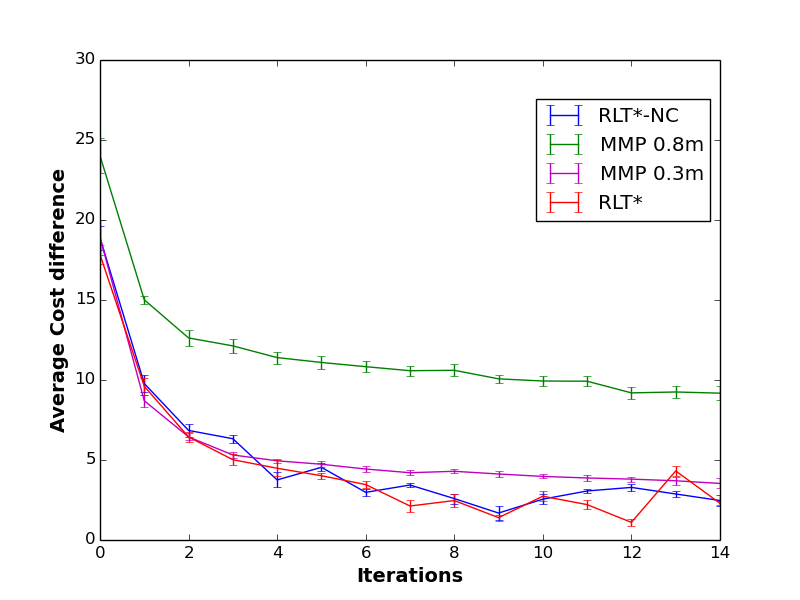
\includegraphics[clip=true,width=1.\textwidth]{figures/cost_diff_train.png}
    \caption{Train}
    \label{fig:train_results}
  \end{subfigure}
 % \hspace{5mm}
  \begin{subfigure}[b]{0.45\columnwidth}
    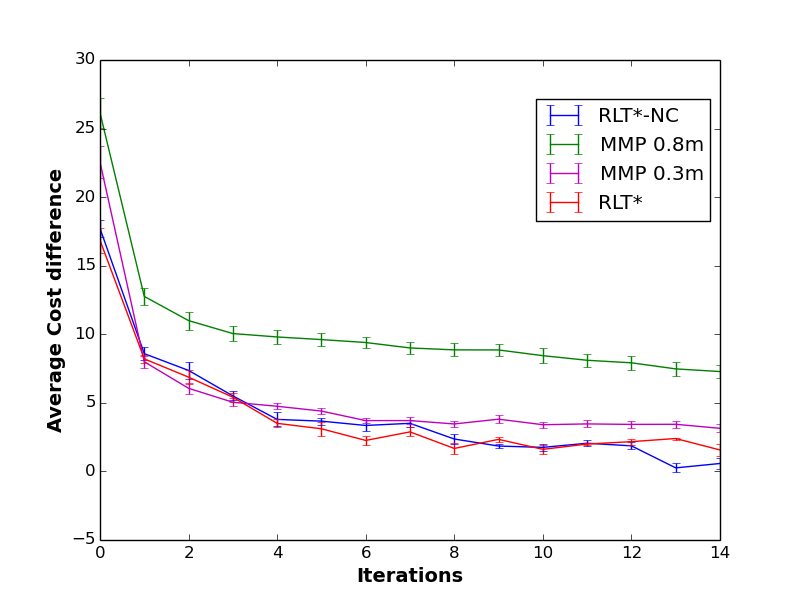
\includegraphics[clip=true,width=1.\textwidth]{figures/cost_diff_val.png}
    \caption{Test}
    \label{fig:test_results}
  \end{subfigure} 

  %\vspace{-3mm}
  \caption[Train and test set average cost difference, for 15 iterations.]{Train and test set average cost difference, for 15 iterations. Error bars represent standard error over four independent runs on shuffled versions of the data. (RLT$^*$-NC is RLT$^*$ without caching.)}
  %\vspace{-3mm}
  \label{fig:results}
\end{figure}



	\begin{table}[]
  \centering
	\scalebox{1.}{
	\begin{tabular}{|l|l|l|l|l|}
	\hline
	               & MMP$_{0.8}$     & MMP$_{0.3}$       & RLT$^*$-NC  & RLT$^*$ \\ \hline
	Iteration (s) & 1.83(0.79) & 20.93(12.14) & 12(0) & 5.87(0.50)  \\ \hline
	Learning (s) & 275.2      & 3140.6       & 1808  & 911.7       \\ \hline
	$Q(\zeta,\zeta_i,\mathbf{w}_{gt})$ & 7.28      & 3.14       & 0.57  & 1.57       \\ \hline
	\end{tabular}}
	\caption[Per iteration and total learning times.]{Per iteration and total learning times for our proposed algorithms and the baselines (RLT$^*$-NC is RLT$^*$ without caching.). Values in parentheses denote standard deviation.}
	\label{tab:time}
	\end{table}


	\begin{figure}
	\centering
	%\vspace{-3.3mm}
	    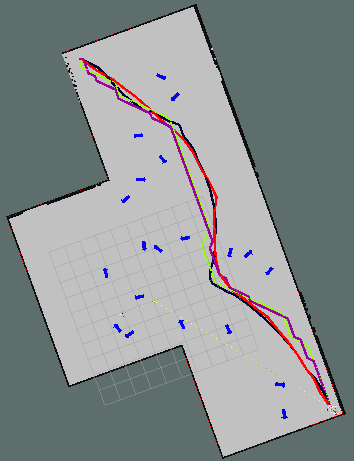
\includegraphics[width=0.3\textwidth]{figures/path_compare.png}
	%\vspace{-4mm}
	  \caption[Qualitative comparison of paths.]{Qualitative comparison of paths. Goal is at the top left, robot begins on the bottom right. Black: demonstration path. Red: RLT$^*$. Green: MMP$_{0.8}$, Magenta: MMP$_{0.3}$ }
	  \label{fig:path_compare}
	\end{figure}


	\begin{figure}[tbh]
	\hspace{5mm}
      \begin{subfigure}[b]{0.309\columnwidth}
    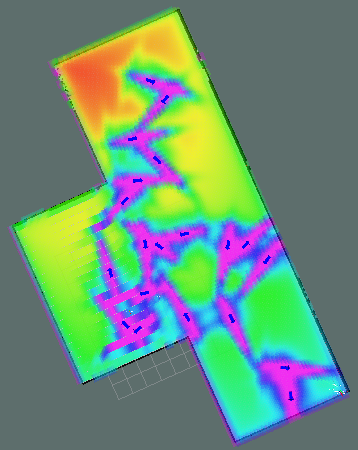
\includegraphics[width=1.\textwidth]{figures/gt_ct.png}
    \caption{Ground truth}
    \label{fig:get_cf}
  \end{subfigure}
  %\hspace{1mm}
  \begin{subfigure}[b]{0.30\columnwidth}
    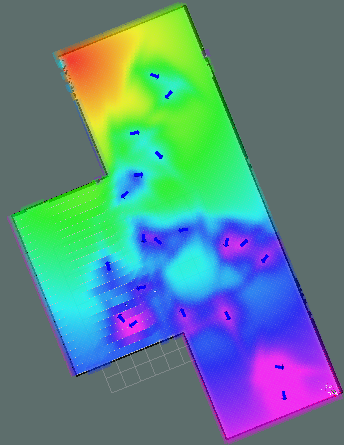
\includegraphics[width=1.\textwidth]{figures/astar03.png}
    \caption{MMP$_{0.3}$}
    \label{fig:astar03_cf}
   \end{subfigure}
   %\hspace{1mm}
  \begin{subfigure}[b]{0.305\columnwidth}
    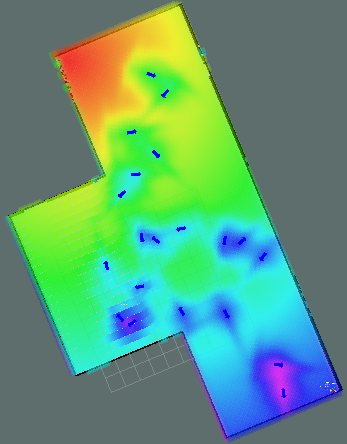
\includegraphics[width=1.\textwidth]{figures/rrt_cf.png}
    \caption{RLT$^*$}
    \label{fig:rrt_cf}
  \end{subfigure} 
  	  \caption{Ground truth and learned cost functions using MMP$_{0.3}$ and RLT$^*$.  \label{fig:cfs}}
  \end{figure}


\subsection{Conclusion and Future Work}
In this section, we proposed Rapidly Exploring Learning Trees (RLT$^*$), which learns the cost functions of Rapidly Exploring Random Trees (RRT) from demonstration, thereby making inverse learning methods applicable to more complex tasks. Our approach extends the Maximum Margin Planning to work with RRT$^*$ cost functions. Furthermore, we proposed a caching scheme that greatly reduces the computational cost of this approach. Experimental results on real and simulated data from a social navigation scenario showed that RLT$^*$ achieves better performance at lower computational cost than existing methods.

 Although our experimental comparison used A$^*$ as a baseline, RLT$^*$ is also well suited to situations where deterministic planners naturally fail, e.g., a manipulator with many degrees of freedom. A clear avenue for future work is to design learning algorithms that explicitly take into account the probabilistic nature of RRT$^*$. We also plan to evaluate RLT$^*$ on data using the actual TERESA robot. This will in turn allow us to deploy the learned cost function on the robot. Finally we will combine learning from failure, introduced in Section \ref{sec:irlf} with the RLT$^*$ and evaluate its performance on the TERESA robot.

\clearpage





\section{Learning Body Pose Policies from Demonstration}
\label{sec:sl_policy}

Apart from being able to navigate socially, a key functionality for our semi-autonomous telepresence system, is to allow the pilot to engage in conversation 
with the people around the robot, without any input from the pilot himself. While in some ideal conditions this would be a simple tracking problem, it is no longer the case in real social environments. This is because firstly there could be significant sensor noise, not allowing the robot to track everyone in its surroundings. Secondly, in crowded environments social norms become harder to hard code. The TERESA system attempts to deal with these problems by learning from human interaction.

In Deliverable 5.3 we described in detail, several experiments of people and groups interacting with the robot. During these interactions both the pilot and the interaction target(s) gave direct feedback on the robots behaviour. After processing the collected data, two cost functions were produced that allowed us to encode people's prefferences with respect to the robot. In this deliverable we take a different approach. Instead of asking direct feedback from users we employ a human expert to demonstrate the correct behaviour to the robot. Using the collected demonstrations we learn a direct mapping from sensor readings to socially appropriate actions. The rest of the section is organised as follows. 

\begin{itemize}
	\item In Section \ref{sec:initial_experiment} we describe local experiments performed at the UvA. The aim of this experiments where to simulate different social situations and extract human demonstrations of control during robot conversation. We further describe how this data was filtered and processed.
	\item In Section ?? we describe the use a Deep Neural Network architecture to learn a robust social conversation policy from the collected data. 
	\item Finally in Section ?? we perform an evaluation of our resulting system.
\end{itemize} 

The reasoning behind our approach is described in more detail in Deliverable 5.4. 

\subsection{Local Experiments and demonstration collection}
\label{sec:initial_experiment}
The fist step to achieving the goals set out in this section was to perform experiments in order to collect appropriate demonstration data in various social interaction situations. These experiments took place at the University of Amsterdam in August 2016. These were focused on collecting control data from human demonstrations at different social situations as well as data from all of the robot's sensors. Using machine learning, the aim was to match sequences of input data to the appropriate controls allowing the robot to thus mimic the human demonstrations in new unseen situations. The main aims of the experimental setup and procedure were:

\begin{itemize}
\item To collect data of the robot interacting with various groups sizes.
\item To impose siginificant variability in the sensor and demonstration data 
\end{itemize}

\subsubsection{Experimental Setup}
The setup of this experiment is similar to the one used in the previous deliverable and is depicted in figure ??. The TERESA robot is placed along with four interaction targets into the "interaction room". Three of the interaction targets are volunteers and vary with each experimental session while one is a researcher from the project. During the experimental session the interaction targets interact with the robot in a social manner. 

The researcher also participates in the interaction but has the additional role of inducing different social situations such that sufficient variability in the data is ensured. This was done by instructing the volunteers to:

\begin{itemize}
 	\item Leave or join the group.
 	\item Sit down or stand up.
 	\item Move
 	\item Change group formation.
\end{itemize}
 Meanwhile in the "control room" another researcher acts as an expert demonstrator, controling the TERESA robot and making sure that the interaction is socially appropriate. 

The following was collected during our experiments:

\begin{itemize}
	\item Linear and angular velocity ($v,\omega$) commands, generated by the expert. 
	\item Person positions  ($x,y$) as detected by the robot's on board localisation module.
	\item Ground truth person positions ($x_{gt},y_{gt}$) using the Optitrack overhead tracking system.
	\item Laser and RGBD sensor data.
	\item Odometry.
\end{itemize}

\subsubsection{Processing}

Before using a learning algorithm to learn a mapping from sensor observations to linear and angular velocities, the collected data was first filtered and processed into an appropriate representation. 

The first step in processing was removing parts where we would not expect the robot to learn a correct mapping for. This occured for example in cases where the participants would quickly move away from the robot, in cases where unusual circumstances took place, or times when the human expert would make an obvious mistake. This data filtering took place by playing back the data and annotating frames where innapropriate data was present, so that they could be ingored further down the pipeline. 

Next using the ground truth data from the Optitrack system we labeled which person was considered to be the interaction target during the conversation. This step is essential because during normal use of the TERESA system an interaction target also needs to be defined by the pilot. The ground truth positions of the interaction targets was not used to correct the readings from the robots localisation system. This ensured that during learning we also learn a model of the localisation system`s noise. 

After filteting the next step was data synchronisation. During the experiments the data from the localisation system and control come at different rates and are thus asynchronous. We synchronised the data by first setting the desired control rate for the final system at 10Hz and then retrieving the latest data from the localisation system and the control outputs at that rate.   

At this point out data consisted of:
\begin{itemize}
	\item Inputs: N Tracked person positions at time t, $\{[x_1,y_1],[x_2,y_2] .., [x_N,y_N]\}_t$
	\item Outputs: Angular and linear velocity at time t, ${v,w}_t$
\end{itemize}

A naive approach to the problem would attempt to learn a direct mapping from observations at time $t$ to actions at time $t$. This would have very limited chances of success for many reasons. The observations at a single timestep are not only noisy but also cannot encode context information such as the velocity and acceleration of the tracked persons. It is thus required that we augment the input vector to the learning algorithm with past time $\tau$ time instances. The input vector would thus become a concatenation of all tracked person vectors from time $t- \tau$ to $t$ $\{[x_1,y_1],[x_2,y_2] .., [x_{N_{t-\tau}},y_{N_{t-\tau}}]\}_{t-\tau},.. \{[x_1,y_1],[x_2,y_2] .., [x_{N_t},y_{N_t}]\}_t$ and the output would remain to be angular and linear velocity at time t.

Another problem with our input data is that the number of tracked persons at each time step varies. This variability in the input data makes processing using conventional Machine Learning methods difficult. One way to combat this problem is to set a max number of tracked people at each timestep, $N_max$. We would then make sure to include the closest $N_max$ tracked persons at each time. If $N_t$ would be less than $N_max$ then we could pad that vector with zeros. While this would be a viable option it could pose several difficulties for learning in practice. As an example picture two successive frames with different number of people. We to ensure that past frames are constant we would have to make sure that if a person is the same in the two time slots they should be put into the same person slot in order to facilitate learning, this could make data hard to preprocess and still lead to mistakes. For this reason we take a slightly different approach. For each input vector at time t we create an image such as the one shown in Figure ??. Each person is drawn onto the image as a circle with intensity 1 while the interaction target is drawn as a circle with intensity 2. The position of this circles is determined by the person positions with respect to the robots frame. The created image has a fixed size and resolution which means that it can only represent persons that are present at a maximum distance of $d$ from the robot. In our $d$ was set to 2.5m. Other settings for the created image were as follows:

\begin{itemize}
	\item Resolution:
\end{itemize}

Another advantage of the image representation is that it allows us to use state of the art machine learning methods that exploit spacial structure in images such as convolutional neural networks which have proved to be very effective in image processing tasks. This is explored in the next section.

\subsubsection{Outputs}
The learning algorithm is expected to output a policy, i.e. a control output for a set of inputs. While our outputs are linear and angular velocities, it is not clear wether having continuous or discrete outputs is better in terms of learning and performance of the resulting policy. Having discrete outputs results in a classification problem which is typically easier to solve than a regression problem, which is the case with a continuous representation. Another drawback of continuous representations is that the output distribution could be mutimodal, which is something that continuous output networks do not typically account for. However a continuous representation is much more natural in this case and could result in a much more aggreable behaviour from the robot. For this reason we decided to try both representations and choose best one after deployment on the robot. 

Another problem in terms of the outputs, for this specific application sourced from the fact that during the training data, the robot was stopped for far longer than it was actually moving. This posed problems in both the cases of a continuous and a discrete output. In the discrete case, far more datapoints where in the specific class of $(v,\omega) = (0,0)$ than any of the other individual classes, this can hurt the learning or even urge the network to simply output that class if sufficient measures are not taken. In the continuous case, it may cause the network to output smaller velocities than required. To combat this effect we took two measures. First we made sure that a similar portion of static and moving outputs where present in the data. Secondly we experimented with a hierarchical output architecture. In this case, the learning algorithm must first clasify wether or not the output should be (0,0) or something else. Then given that the output is not (0,0) it decides what the output should be. This feature made a big difference when deployed on the robot and it is hence present in all the models we consider.



In fact the two are very hard to compare numerically appart from how the policy actually looks. 
 

\subsection{Learning}

In the previous section we explained how the data of person positions at each timestep was processed to allow learning. We also reasoned that an image representation such as the one shown in Figure ?? would be more appropriate. We further argued that the learning procedure would be much more effective if the evolution of these images over time was to be taken into account. In this section we use these two key points to construct a deep neural network (DNN) architecture in order to learn the mapping.

\subsubsection{Convolutional Layers}
Convolutional neural networks have been particuarly effective in extracting useful features from static images. Input to a convolutional layer is an image $n_ixn_i$ image with $c_i$ channels. The input convolved by a set of $k$ filters of dimentions $n_f \times n_f$, resulting in $k$ output feature maps that are then subject to a non-linearity and possibly a subsampling operation. The result of the computation can then be considered a new image of $k$ channels and dimention $n_1xn_1$. This procedure may thus be repreated for many layers of computation. A key aspect of convolutional networks is that the filter weights (or shapes) are learned. This means that they can be trained to extact the image features usefull for the specific application. 

\subsubsection{Long Short Term Memory}
Recurrent neural network architectures allow DNNs to deal with input sequences instead of simply static inputs.
In contrast to fully connected and convolutional networks, an RNN allows the network to retain a state based on its previous inputs. This is done by essentially feeding back to the network a representation of the previous inuput. This makes them ideal in dealing with time varying and variable length inputs. An outline of an RNN is shown in Figure ??.
  
Long short term memory networks (LSTM) are the defacto standard architecture for Recurrent Neural Networks (RNN). While the general architecture follows the one shown in Figure ??, the way that the feedback and output of the network are computed is especially designed to prevent the gradients of the network from exploding or becoming to small. This has allowed LSTMs to excell in various sequance prediction tasks such as handwriting and speech recognition. 

We have argued in the previous section, that it would be very hard to learn a mapping from inputs to demonstrations if the robot would have no memory of past input states (images). This is because, simply put, the environment is partially observable. Using the LSTMs allows us to use past inputs, which in turn allows it to disambiguate between different input images and makes it more robust to the person localisation system`s false possitives. 

\subsubsection{Architecture}

The overall architecture of the DNN we used is depicted in Figure ??. The current image at time $t$, $s_t$ is input to the system. This is then processed by two convolutional layers using kernels of size $5\times5$ resulting to 15 feature maps at each layer. At each layer the feature maps are subsampled by 2, so that the filters may operate at different scales. The output of the second convolutional layer is flattened and is input two LSTM layers. Finally using a fully connected network we reduce the output of the final LSTM network to the required dimentionality. The architecture is further visualised in Figures ??  and ??. Being fully differentiable the network is trained using backpropagation. 


\subsection{Results}

\section{Integrating cost functions and human demonstrations}


\section{Conclusions and Future Work in Tasks 5.1 and 5.2}
\label{sec:conclusions}
This deliverable has summarised our progress for Work Package 5 from month 15 of the project until month 30. Significant progress has been achieved in all aspects of social behaviour learning on the TERESA robot. 

 An important aspect of this progress is in terms of learning from human demonstrations, using IRL. Firstly we have enabled the robot to learn from failed demosntrations as well as succesful ones in a unified principled framework. We have demonstrated that our method is capable of utilising the failed demonstrations in conjunction with the succesful ones to learn faster and better. Secondly we have developed a novel IRL method called, RLT$^*$ that works with RRT$^*$ as the underlying planner. RRT's are at the heart of TERESA's path planning module, thus learning directly using this planners is bound to produce superior learning results. We have also shown that our method is faster and better that a similar method that uses deterministic planners. A clear avenue of future work is to deploy RLT$^*$ on the real system. Furthermore we plan to integrate these methods together and evaluate any improvement on the real system.

 We have also reported significant progress in terms of experimentation and implementation of social conversation policies. Specifically, we conducted experiments and performed the necessary analysis, in order to discover a cost function for the distance between the robot and the interaction target. In addition we performed statistical analysis on an existing dataset gathered by our partners at UT. This dataset consisted of groups of people scoring how well the TERESA robot approached them. This analysis allowed us to produce a second cost function that determines how the robot should be orientated in such situations. The analysis also concluded that the bearing of the robot to the group's geometric centre was far more important to the bearing with respect to an individual person. This allowed us to determine a compact yet representative state-space representation for the robot during conversation. 

In terms of social conversation, there are three directions of future work we are currently pursuing, and for which we plan to report in month 36. Firstly, we aim to apply the methods for IRL that were here presented to the problem of learning social cost functions for social conversation from expert demonstrations of the interaction behaviors; Secondly, we aim to integrate the available cost functions in order to learn a single social conversation policy under which the robot operates. Finally, we aim to make the resulting policy more robust to false positives from the robots social detectors using advanced filtering techniques such as \emph{partially observable Markov decision processes} (POMDPs) and \emph{long-short memory networks} (LSTMs).

\bibliographystyle{plain}
\bibliography{references}

\end{document}
